\subsection{Associazioni}

\begin{definition}[Istanza di un'associazione]
    Un'istanza di un'associazione determina un legame logico tra due o più istanze.
\end{definition}

\begin{definition}[Associazione]
    Un'associazione $R(X, Y)$ fra due collezioni di entità chiamate $X$ e $Y$
    è un insieme, che varia nel tempo, di istanze di associazione tra gli elementi delle due collezioni.
    Il prodotto cartesiano $(X \cdot Y)$ è chiamato \textcolor{purple}{dominio dell'associazione}.
\end{definition}

Un'associazione è caratterizzata da due proprietà: \textcolor{purple}{molteplicità} e \textcolor{purple}{totalità}.

\begin{definition}[Vincolo di Unicità]
    Un'associazione $R(X, Y)$ è detta \textcolor{purple}{univoca}
    rispetto ad $X$ se per ogni elemento di $x \in X$ esiste al più un elemento
    $y \in Y$ che è associato ad $x$. Se questo vincolo non vale, si dice che l'associazione
    è \textcolor{purple}{multivalore} rispetto ad $X$.
\end{definition}

\paragraph{Cardinalità dell'Associazione}

\begin{itemize}
    \item $R(X, Y)$ è \textbf{\textcolor{purple}{(1:N)}} se è multivalore sy $X$ ed univoca su $Y$.
    \item $R(X, Y)$ è \textbf{\textcolor{purple}{(N:1)}} se è univoca sy $X$ e multivalore su $Y$.
    \item $R(X, Y)$ è \textbf{\textcolor{purple}{(N:M)}} se è multivalore sy $X$ e multivalore su $Y$.
    \item $R(X, Y)$ è \textbf{\textcolor{purple}{(1:1)}} se è univoca sy $X$ ed univoca su $Y$.
\end{itemize}

\begin{definition}[Vincolo di Totalità]
    Un'associazione $R(X, Y)$ è detta \textcolor{purple}{totale} su X se per ogni elemento
    $x \in X$ esiste almeno un elemento $y \in Y$ associato ad $x$. Se questo vincolo non vale,
    si dice che l'associazione è \textcolor{purple}{parziale} rispetto ad $X$.
\end{definition}

\newpage
\paragraph{Rappresentazione delle Associazioni} Un'associazione fra due collezioni $C_1$ e $C_2$ si rappresenta
con una linea che collega le due classi. La linea si etichetta con il nome dell'associazione. L'\textcolor{purple}{univocità}
di una classe $C_1$ si rappresenta disegnando una freccia singola sulla linea che esce và da $C_1$ a $C_2$. Se invece l'associazione è
\textcolor{purple}{multivalore} si indica con una doppia freccia.
La \textcolor{purple}{parzialità} invece è rappresentata con un taglio sulla linea vicino alla freccia, mentre la
\textcolor{purple}{totalità} è rappresentata dall'assenza del taglio.

\begin{figure}[h]
    \centering
    \captionsetup{justification=centering}
    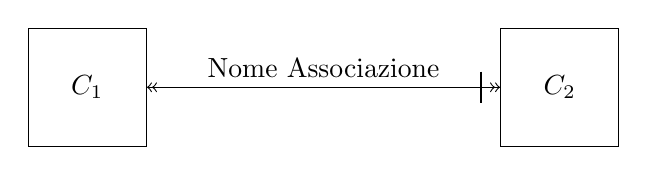
\begin{tikzpicture}[node distance=6cm, scale=2, main/.style={rectangle, draw, minimum size=15mm}]
        \node[main] (1) {$C_1$};
        \node[main] (2) [right of=1]{$C_2$};
        \draw[<<->>] (1) -- (2) node[midway, above] {Nome Associazione};
        \draw (2.5, 0.1) -- (2.5, -0.1);
    \end{tikzpicture}
    \caption{In questo caso abbiamo un'associazione \emph{multivalore} da entrambe la parti, ma \emph{parziale} per $C_2$ e \emph{totale} per $C_1$}
\end{figure}

\begin{figure}[h]
    \centering
    \captionsetup{justification=centering}
    \begin{tikzpicture}[node distance=4cm, scale=2, main/.style={rectangle, draw, minimum size=15mm}]
        \node[rectangle split, rectangle split parts=2, draw] (prop) {Nome Associazione \nodepart{second} Proprietà};
        \node[main] (1) [below left of=prop]{$C_1$};
        \node[main] (2) [below right of=prop]{$C_2$};
        \draw[<->>] (1) -- (2);
        \draw (0.9, -1.3) -- (0.9, -1.55);
        \draw[dashed] (0, -1.4) -- (prop);
    \end{tikzpicture}
    \caption{Le associazioni possono presentare \textcolor{purple}{proprietà}}
\end{figure}

\begin{figure}[h]
    \centering
    \captionsetup{justification=centering}
    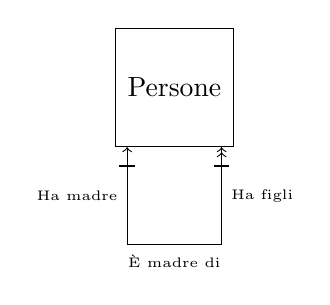
\begin{tikzpicture}[node distance=4cm, scale=2, main/.style={rectangle, draw, minimum size=15mm}]
        \node[main] (1) {Persone};
        \draw[->] (-0.3, -1) -- (-0.3, -0.38) node[midway, left] {\tiny{Ha madre}};
        \draw[->>] (0.3, -1) -- (0.3, -0.38) node[midway, right] {\tiny{Ha figli}};
        \draw[-] (-0.3, -1) -- (0.3, -1) node[midway, below] {\tiny{È madre di}};
        \draw[-] (-0.35, -0.5) -- (-0.25, -0.5);
        \draw[-] (0.25, -0.5) -- (0.35, -0.5);
    \end{tikzpicture}
    \caption{O possono anche essere \textcolor{purple}{ricorsive}}
\end{figure}